\cotefile{87}
\scanpage{29}
\[
C\subset E \qquad
\begin{aligned}
&C\ \text{partie polyédrale de l'espace affine }E\\
&\qquad \dim C=d
\end{aligned}
\]

$A_C=\mathrm{Aff}(C)$ espace affine engendré par $C$

$C^0=\mathrm{Int}_{A_C}(C)$ est la facette maximale (= de dim maximale), $C=\overline{C^0}$.

Les autres facettes \inserted{fermées} sont les intersections \inserted{$H\cap C$ avec $C$} d'hyperplans $H$
de $A_C$ ne rencontrant pas $C^0$ \deleted{\unsure{avec le}}. Les facettes
\deleted{fermées \unsure{telles q|telles que}} de dim $d-1$ correspondent \inserted{$1-1$} aux
$H$ tels que \deleted{\unsure{l'}}l'intérieur de $H\cap C$ dans $H$ soit $\ne\varnothing$,
et les intérieurs en question sont les facettes \inserted{\unsure{ouv}} de
dim $d-1$. Soit $C^1$ leur réunion.

Les facettes fermées de dim $\leq d-2$ sont les int. avec
$C$ de sous-espaces affines de dim $d-2$ de $A_C$ ne
rencontrant pas $C^0\cup C^1\ldots$

Les facettes fermées de dim $\leq d-i$ sont les int.
\inserted{$F\cap C$} avec $C$ des sous-espaces \inserted{\unsure{aff}} $F$ de $A_C$ de dim
$d-i$ \inserted{(i.e. \unsure{codim|codim.} $i$)} qui ne rencontrent pas $C^0\cup C^1\cup\ldots\cup C^{i-1}$.
Les facettes fermées de dim $d-i$ sont en
corr. $1-1$ avec les $F$ tels que $\mathrm{int}_{F}\,F\cap C\ne\varnothing$,
et \inserted{les} $\mathrm{int}_F\,F\cap C$ sont les facettes de dim $d-i$.

Intersection de deux facettes fermées est une
facette fermée [c'est une partie convexe de $C$ et
c'est une réunion de facettes, il reste \unsure{à prouver|: prouver}):

% Vertical pen stroke to the left of the next two manuscript lines.
\uline{Prop} Les facettes \inserted{fermées} de $C$ sont les réunions
de facette qui sont convexes et fermées.

Soit
% archive sheet number: 28

\scanpage{30}
$F$ facette, alors \deleted{$\unsure{F}$} a) $F=\mathrm{int}_{A_F=A_{\overline F}}\overline F$, $\overline F=A_F\cap C=$

\deleted{b) $\overline F$ \unsure{est une} facette,}

b) $F'\subset C$ alors
\[
\begin{aligned}
&\underbrace{F'\ \text{facette de }\overline F}\\
&\hspace{3em}\unsure{\Updownarrow|\Downarrow}\\
&F'\ \text{facette de }C,\ F'\subset F
\end{aligned}
\]
[$\Rightarrow\overline F$ réunion de facettes]

c) Soit \deleted{$F$} $K\subset C$. Pour que $K$ soit \unsure{une} facette
fermée, il f. et S. que $K$ soit convexe, fermé et
une réunion de facettes. ($\Rightarrow$ une intersection
de deux facettes est une facette)

d) \deleted{\unsure{$L$}} Soit $\mathrm{Fac}(C)=\Pi$ \inserted{\unsure{l'ens|l'ens.} ordonné des facettes}. Alors

1°) $\Pi^\circ$ (l'ens. ordonné opposé) est isomorphe
à un ens $\unsure{\mathrm{Fac}'|\mathrm{Fac}}(C')$, où $C'$ est une
\inserted{\unsure{part. polyédriq|partie polyédriq|partie polyédrale}} convexe \deleted{\unsure{fermé}} dans $E$ de $=$ dim.

2°) \deleted{Soient} $F'_{\deleted{\unsure{1}}},F''_{\deleted{\unsure{2}}}\in\Pi$ \inserted{avec $F'<F''$}, $\Pi_{F',F''}$ l'ens ordonné des $F\in\Pi$, tels que $F'\leq \deleted{\unsure{F'}}F\leq F''$. Alors $\Pi_F$
est \inserted{$\simeq$ à un ens ordonné} de la forme \deleted{$\unsure{F}$} $\mathrm{Fac}(K')$, où
$K'$ un \inserted{polyèdre} convexe de dim $\delta=\dim F''-\dim F'-1$

% Short vertical emphasis stroke beside the corollary.
\uline{Cor} Si \deleted{\unsure{on}} $\dim F''-\dim F'=2$, alors \deleted{card} l'ens
des $F$ tels que $F'<F<F''$ est de card. $2$.

\figure{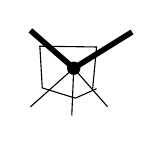
\begin{tikzpicture}[x=1cm,y=1cm]
\draw (-.44,.28)--(.29,.27)--(.24,-.26) (-.43,.27)--(-.4,-.25)--(.02,-.38)--(.29,-.26);
\draw (-.55,-.49)--(0,0)--(.43,-.49) (0,0)--(-.025,-.60);
\draw[line width=2pt] (-.55,.48)--(0,0)--(.74,.46);
\fill (0,0) circle (.085);
\end{tikzpicture}}

\uline{Polyèdre combinatoire} : ens ordonné
fini $I$ satisfaisant les conditions

a) $I$ a des inf et des sup \unsure{quelc}
[plus petit et plus gd élément, et
$i\wedge j$ et $i\vee j$]

b) $I$ satisfait condition des chaines

c) Si $i<j<$\deleted{\unsure{$d$}}$k$ et si $j$ succ. \deleted{\unsure{imméd.|immédiat}} de $i$
$k$ succ. de $j$
% archive sheet number: 29

\scanpage{31}
alors $\exists!\ j'\in I$ tel que
\[
\left\{\begin{aligned}
&j'\ne j\\
&j'\ \text{succ. de }i,\ k\ \text{succ. de }j'
\end{aligned}\right.
\]

\margin{$\downarrow\ \Rightarrow$}
d) \deleted{\unsure{$\forall$|tout}} $i\in I$, \inserted{$i$ non \unsure{minimum|minimal|minimiseur}} \deleted{\unsure{et non plus petit} \unsure{él.} $0$}
\[
\begin{aligned}
&i=\mathrm{Sup}\,(j\in I\mid j<i)\\
&i\ \text{non max-imal.}\Rightarrow \deleted{\unsure{\text{si }i\ne}}\ i=\mathrm{Inf}\,(j\in I\mid j>i)
\end{aligned}
\]

\uline{dim $-1$} \quad $I$ a un seul élément $(0=1)$.

\uline{dim $0$} \quad $I$ a deux éléments distincts ($0$ et $1$, \deleted{\unsure{$\exists$}} $0\ne1$)

\uline{dim $1$} \quad $I$ a \deleted{trois} quatre éléments $0$, $1$ et deux \unsure{int.|incomp.} $x,y$

( \deleted{$x,y$ \unsure{son}}

\diagram{\begin{tikzcd}[ampersand replacement=\&,column sep=small,row sep=small]
 \& 1 \arrow[dl,dash]\arrow[dr,dash] \&\\
 x \& \& y\\
 \& 0 \arrow[ul]\arrow[ur,dash] \&
\end{tikzcd}}

\uline{dim $2$}

\diagram{\(\begin{array}{lll}
\dim -1&0&\\
\dim 0&x_0\quad x_1\ldots x_{n-1}&\\
\dim 1&&\\
\dim 2&1&\begin{array}{l}\text{contours}\\\text{dont les comp.}\\\text{conn. ont au moins 3 sommets}\end{array}
\end{array}\)}

\figure{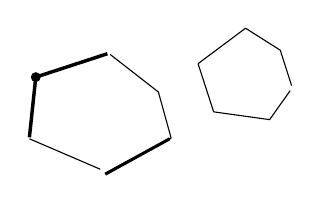
\begin{tikzpicture}[x=.9cm,y=.9cm,line join=round]
\draw[line width=1.25pt] (0,0)--(.09,.85)--(1.1,1.18);
\draw (1.14,1.17)--(1.82,.64)--(2,-.01)--(1.08,-.5);
\draw[line width=1.1pt] (1.07,-.52)--(1.98,-.02);
\draw (0,-.02)--(1,-.45);
\fill (.09,.85) circle (.07);
\draw (2.38,1.04)--(3.05,1.54)--(3.54,1.23)--(3.7,.73);
\draw (3.68,.66)--(3.39,.25)--(2.60,.36)--(2.38,1.04);
\end{tikzpicture}}

\uline{dim $3$} \quad On voudrait que si $x$ est un sommet

\diagram{\(\begin{array}{l|l}
-1&0\\0&\text{sommets}\\1&\text{arêtes}\\2&\text{faces}\\3&1
\end{array}\)}

% Double vertical rule between the table and the following text.
les $y>x$ \deleted{\unsure{qui le} \unsure{contiennent}}, \inserted{$y\ne1$,} forment un
contour \uline{connexe}

et si $x$ est une face
les $y<x$ \unsure{qq|que}, $y\ne0$,
forment un \uline{contour}
$(\pi_0\unsure{\simeq|=}0)$

\uline{dim $4$}
% archive sheet number: 30

\scanpage{33}
a) $\vec A\hookrightarrow S\times A$, \deleted{$\unsure{A|\forall}$} $\vec A\to A$ de rang $2$

a') $A^\uparrow\hookrightarrow A\times F$, \quad $A^\uparrow\to A$ de rang $2$

\diagram{\begin{tikzcd}[ampersand replacement=\&,column sep=tiny,row sep=small]
\&\vec A\arrow[dl]\arrow[dr]\&\&A^\uparrow\arrow[dl]\arrow[dr]\&\\
S\arrow[d,equal]\&\& A\arrow[d,equal]\&\&F\arrow[d,equal]\\
\mathcal X_0\&\&\mathcal X_1\&\&\mathcal X_2
\end{tikzcd}}

b) $A^{\vcenter{\hbox{\tikz[x=.15cm,y=.15cm]{\draw[->] (0,0)--(0,1.2);\draw[->] (0,0)--(1.3,0);}}}}=\vec A\times_A A^\uparrow\to S\times F$ est de rang $2$ sur son image

c) $\forall s\in S$, l'ens $\mathcal X_{\inserted{>s}}\deleted{\unsure{(s)}}$ des $a\in A$ et $f\in F$
incidents à $s$ (qui est un \uline{graphe} de
sommets $A$, d'arêtes $F$, grâce à b), et
\unsure{$=$|$\subset$|$\simeq$} un \uline{contour} grâce à a')) est un
\uline{polygône} (i.e. est un contour \inserted{$\ne\varnothing$} \uline{connexe})

c') $\forall f\in F$, l'ens $\mathcal X_{<f}$ des $a\in A$ et $s\in S$
incidents à $f$ (qui est un \uline{graphe} \ldots{}
grâce à a), et un \uline{contour} grâce à b))
est un \uline{polygône} (i.e. est un contour \inserted{$\ne\varnothing$} \uline{conn.})

Version commune (introduisant $\mathcal X_{-1}=\{\varnothing\}$, $\mathcal X_3=\{1\}$ (plus \unsure{grds|grand}
et plus petit élément)

Si $-1\leq i\unsure{<|\leq}j\leq3$, \inserted{avec} $\delta=j-i\geq2$, et \deleted{\unsure{et}} $(i,j)\ne(-1,3)$, si $x_i\in\mathcal X_i$, $y_j\in\mathcal X_j$,
et $\mathcal X_{i<\,?\,<j}$ est l'ens ordonné des $x\in\mathcal X$ \deleted{$\unsure{<}$} tels que
$x_i<x<y_j$, alors la réalisation topologique de $\mathcal X_{i\leq\,\,\leq j}$ est
homéomorphe à \deleted{$\unsure{\Sigma}$} $\unsure{S|\mathbb S}^{\delta-1}$ (sphère de dim $\delta-1$). [Se
généralise aux polyèdres lisses de dim quelconque, cf plus
bas\ldots]

Les conditions a), a'), b) permettent de définir sur
$A^{\vcenter{\hbox{\tikz[x=.15cm,y=.15cm]{\draw[->] (0,0)--(0,1.2);\draw[->] (0,0)--(1.3,0);}}}}$ les opérations $\sigma_1,\sigma_2$ et $\varepsilon$ [avec $\sigma_1\sigma_2=\sigma_2\sigma_1$ \deleted{\unsure{et}}, soit $\sigma$,
et $\sigma_1,\sigma_2,\varepsilon$ étant des involutions, $\sigma_1,\sigma_2,\sigma,\varepsilon$ étant ss
pts fixes ---] les conditions c), c') assurent que
$S,F$ ``sont'' bien les ens de sommets et des faces de la
carte lisse combinatoire ainsi définie\ldots
% archive sheet number: 32

\scanpage{34}
On trouve ensuite

$\widetilde S=A^{\vcenter{\hbox{\tikz[x=.15cm,y=.15cm]{\draw[->] (0,0)--(0,1.2);\draw[->] (0,0)--(1.3,0);}}}}/\rho_s\simeq$ ens des couples $(s,\omega)$, $s\in S$, $\omega$ une orientation du \deleted{\unsure{lien}}
polygône $\mathcal X_{\geq s}$ des $a\in A$ et $f\in F$ incidents à $s$
[i.e. un \inserted{des 2} ordres circulaires sur l'ens des $a\in A$ incidents à $s$, qui définissent sa structure polygonale]

$\widetilde F=A^{\vcenter{\hbox{\tikz[x=.15cm,y=.15cm]{\draw[->] (0,0)--(0,1.2);\draw[->] (0,0)--(1.3,0);}}}}/\rho_f=$ ens des couples $(f,\unsure{\varpi|\bar\omega})$, $f\in F$, $\varpi$ une orientation du
polygône $\mathcal X_{\leq f}$ des \deleted{$\unsure{f}$} $a\in A$ et $s\in S$ incidents à $f$,
[i.e. un des 2 ordres circ. sur l'ens. des
$a\in A$ incidents à $f$, qui définissent sa structure polygonale]

$\widetilde A=A^{\vcenter{\hbox{\tikz[x=.15cm,y=.15cm]{\draw[->] (0,0)--(0,1.2);\draw[->] (0,0)--(1.3,0);}}}}/\sigma=$ ens des couples $(a,u)$, $a\in A$, $u\in\vec A(a)\wedge A^\uparrow(a)$,
où $\vec A(a)$ ($A^\uparrow(a)$) est l'ens des \unsure{axes|arcs|sens} tang.
(axes transverses) portés par l'arête $a$.

\[
A^\wedge=\mathrm{Im}\,(A^{\vcenter{\hbox{\tikz[x=.15cm,y=.15cm]{\draw[->] (0,0)--(0,1.2);\draw[->] (0,0)--(1.3,0);}}}}\to S\times F)
=\begin{aligned}[t]&\text{rel. d'incidence}\\&\text{entre }S\text{ et }F\end{aligned}
\]

\diagram{\begin{tikzcd}[ampersand replacement=\&,row sep=large,column sep=small]
\&\& A^{\vcenter{\hbox{\tikz[x=.15cm,y=.15cm]{\draw[->] (0,0)--(0,1.2);\draw[->] (0,0)--(1.3,0);}}}} \arrow[dll,"\rho_s"']\arrow[dl,"\unsure{\sigma_2|\sigma}"']\arrow[d,"\sigma" description]\arrow[dr,"\sigma_1"]\arrow[drr,"\rho_f"]\&\&\\
\widetilde S\arrow[d,"\sigma_1"']\&\vec A\arrow[dl]\arrow[dr,"\sigma_1"']\&
\widetilde A\arrow[d,"\sigma_1"',"\sigma_2"]\&A^\uparrow\arrow[dl,"\sigma_2"]\arrow[dr]\&\widetilde F\arrow[d,"\sigma_2"]\\
S\&\&A\&\&F
\end{tikzcd}}

\[
\begin{aligned}
A^{\vcenter{\hbox{\tikz[x=.15cm,y=.15cm]{\draw[->] (0,0)--(0,1.2);\draw[->] (0,0)--(1.3,0);}}}}&\simeq\widetilde S\times_S\vec A\simeq\deleted{\unsure{\widetilde F}\times_F}A^\uparrow\times_F\widetilde F\\
&\simeq\vec A\times_A A^\uparrow\\
&\simeq\vec A\times_A\widetilde A\simeq\widetilde A\times_A A^\uparrow\\
&\simeq\widetilde S\times_S A^\wedge\simeq A^\wedge\times_F\widetilde F
\end{aligned}
\]

\diagram{\begin{tikzcd}[ampersand replacement=\&,row sep=small,column sep=small]
\&A^{\vcenter{\hbox{\tikz[x=.15cm,y=.15cm]{\draw[->] (0,0)--(0,1.2);\draw[->] (0,0)--(1.3,0);}}}}\arrow[dl]\arrow[d]\arrow[dr,dash]\&\\
\widetilde S\arrow[d]\&A^\wedge\arrow[dl]\arrow[dr]\&\widetilde F\arrow[d,dash]\\
S\&\&F
\end{tikzcd}}

$A^{\vcenter{\hbox{\tikz[x=.15cm,y=.15cm]{\draw[->] (0,0)--(0,1.2);\draw[->] (0,0)--(1.3,0);}}}}$ s'identifie aux rel. d'incidences
\[
\begin{aligned}
&\text{entre }(S,A,F)\quad\text{simultanément}\\
&\text{entre }\widetilde S,\widetilde A,\\
&\text{entre }\widetilde A,\widetilde F,\\
&\text{entre }\widetilde S,\widetilde F,
\end{aligned}
\]
% archive sheet number: 33

\scanpage{35}
Explicitons l'axiome

D) Toute \deleted{\unsure{ens}} \inserted{partie} minorée \inserted{$\ne\varnothing$} \deleted{\unsure{d'éléments}} \inserted{de $\mathcal X_{\unsure{**|xx}}=\mathcal X_0\cup\mathcal X_1\cup\mathcal X_2$} admet un inf,
($\Longleftrightarrow$ toute partie majorée \inserted{$\ne\varnothing$} de $\mathcal X_{**}$ admet un sup).

\deleted{Comme il résulte de c) que les él. minimaux de $\mathcal X_{**}$ sont
les él. de $S$, les parties minorées de $\mathcal X_{**}$ sont celles
contenues dans un $\mathcal X_{\geq s}$. Or comme ce dernier
c'est un polygône \inserted{(avec plus petit él.)}, et dans un \inserted{tel} polygône \unsure{satisfaire|satisfaire à|satisfait} la
condition \inserted{d'existence} de borne inférieure \unsure{sss|ssi|ses} \deleted{\unsure{il a au}} son nb de
côtés est $\geq3$ (dans le cas excluant celui $n=2$ ici\ldots)
Donc la condition D se récrit :

d) $\forall s\in S$, il y a au moins trois arêtes \inserted{$a\in A$} incidentes à $s$.}

Il suffit d'exprimer que deux él. distincts \inserted{minorisés \unsure{égalts|dgts|distincts}} de $\mathcal X_{**}$ \deleted{\unsure{ont}} \inserted{majorant un él. de \unsure{$S$}} un inf. Si l'un des deux est $\in\mathcal X_0$ (i.e. est minimum)
c'est trivialement satisfait. Il reste à traiter $3$ cas

1°) \uline{Deux arêtes} : on trouve que 2 arêtes qui ont \unsure{ms|m\textsuperscript{es}}
sommets sont égales, i.e. $(S,A,\vec A)$ est un graphe strict.

2°) \uline{Deux faces} : on trouve \deleted{\unsure{deux faces qui|qu'elles} $(F,A,A^\uparrow)$} \inserted{que les deux faces distinctes}
ont en commun deux sommets, \deleted{\unsure{elles|elles-mêmes}} ceux-ci sont liés
\deleted{\unsure{par une arête qui leur soient}} et elles \deleted{\unsure{ont}} ont en commun l'arête qui les joint,
\inserted{et pas d'autre sommet}

3°) Une arête \inserted{$a$} et une face \inserted{$f$} \deleted{non} \inserted{une arête} incidente --- mais
ayant un sommet commun : \deleted{il faut} exprimer
que le deuxième sommet de $a$ n'est pas dans $f$,
ou encore \deleted{que} : si $f$ est incidente aux
deux sommets d'une arête, elle est incidente
à l'arête.

Regroupant, on trouve

\margin{toute arête est le sup de l'ens de ses 2 extrémités}
$d_1)$ Une arête est déterminée par \deleted{ses} \inserted{l'ens de ses} deux extrémités

$d_{\unsure{2}})$ Une face qui cont les 2 extr. d'une arête contient celle-ci

\margin{toute arête est le Inf de l'ens des deux faces incidentes}
$\unsure{d_1|d'_1})$ Une arête est déterminée par l'ens des deux
faces incidentes

$d'_2)$ Les deux faces incidentes à une arête n'ont d'autre
sommet incident commun que ses extrémités
% archive sheet number: 34

\scanpage{36}
[ $\mathcal X$ ens ordonné, $A\subset\mathcal X$, $B$ l'ens des $b\in\mathcal X$ qui majorent $A$

\deleted{\unsure{$\exists$}} Par définition, $\mathrm{Sup}_{\mathcal X}A$ existe \unsure{sss|ssi} $B$ a un plus petit élément $\beta$,
et on pose \deleted{$\unsure{\beta=}$} $\mathrm{Sup}_{\mathcal X}A=\beta$. Si p. ex. $A$ est vide, $B=\mathcal X$, et
$\mathrm{Sup}_{\mathcal X}\varnothing$ existe sss $\mathcal X$ a un plus petit élément (qui
est alors $\mathrm{Sup}_{\mathcal X}\varnothing$). On \unsure{définit|definit} dualement $\mathrm{Inf}_{\mathcal X}A$\ldots

\uline{Prop. 1} Si $A$ a un plus grand élément $\alpha$, il a un sup. et c'est $\alpha$. (Trivial)

\uline{Prop} 2 Pour que $\mathrm{Sup}_{\mathcal X}A$ existe, i.e $B$ ait un plus petit
él., il f et s que $\mathrm{Inf}_{\mathcal X}B$ existe, et alors
$\mathrm{Inf}_{\mathcal X}B=\mathrm{Sup}_{\mathcal X}A$. c'est évidemment néc \deleted{\unsure{q}} d'après prop. 1. Suff?

Soit $\widetilde A$ l'ens des $a\in\mathcal X$ qui minorent $B$. Donc
$A\subset\widetilde A\unsure{\prec|<}B$. Par hypothèse, ($B$ admet un Inf) $\widetilde A$ a un
plus grand él. $\alpha$, lequel majore donc $\widetilde A$ et a fortiori
$A$, donc $\alpha\in B$, et étant dans $\unsure{\bar A|\widetilde A}$ il minore $B$, donc il
est un plus petit él. de $B$, cqfd.

\uline{\deleted{\unsure{Prop}} Cor} Si tte partie de $\mathcal X$ admet un Inf, alors tte
partie de $\mathcal X$ admet un Sup, et réciproquement.

Si tte partie \deleted{non vide} minorée \inserted{(resp. non vide)} de $\mathcal X$ admet un
Inf, alors tte partie non vide (resp. majorée) de
$\mathcal X$ admet un Sup, et réciproquement. Donc
pour que tte partie min. non vide de $\mathcal X$ admette
un Inf, il f et s que tte partie majorée non
vide de $\mathcal X$ admette un Sup. \hfill]
% archive sheet number: 35

\scanpage{37}
Montrons que l'axiome $D=d)+d')$ implique

\uuline{Corollaire} 1 (moyennant l'axiome D) pour \unsure{tte|tt} $s\in S$,
\deleted{\unsure{on}} $p(s)=\mathrm{Card}\,(A\{s\}=\{a\in A\mid a\geq s\}$ \deleted{$\geq3$} $\unsure{\geq3|\geq2}$ et pour
tout $f\in F$, $q(f)=\mathrm{Card}\,(A\unsure{\}|\{}f\}=\{a\in A\mid a\leq f)\geq3$.

En effet, \deleted{si on avait} $p(s)\ne0$, en vertu de
c). Si on avait $p(s)=1$, on aurait par c) une
seule face incidente à l'\inserted{unique} arête $a$ incidente à $s$,
% slanted
\margin{\uline{NB} $p(s)\geq2$ est \unsure{indépendant|indépendt} de D, de \unsure{$=$|m\textsuperscript{me}} $q(f)\geq2$.}
contrairement à b). Si on avait $p(s)=2$, en vertu
de c) les deux arêtes issues de $s$ seraient incidentes
simultanément aux deux faces incidentes à $s$,
contrairement à $d'_1)$. Donc $p(s)\geq3$. La relation
$q(f)\geq3$ s'établit de même.

\uline{Corollaire 2} (moyennant l'axiome D) : toute face
$f\in F$ est le sup de l'ens de ses sommets,
et le sup de l'ens de ses arêtes.

Tout sommet est le inf de l'ens des
faces qui y sont incidentes, et le
Inf de l'ens des arêtes incidentes.
% archive sheet number: 36

\scanpage{38}
% archive sheet number: 37
\deleted{Soit} $\mathcal X$ ens. ordonné fini (on ne suppose pas qu'il
ait un plus petit ou plus grand élément). On
note \inserted{$|\mathcal X|=$} réal. $(\mathcal X)$ sa réalisation topologique (avec sa
décomposition \unsure{cônique|conique} canonique, permettant
d'identifier $\mathcal X$ à un ens ordonné de parties
fermées de $\mathcal X$ \inserted{recouvrant $\mathcal X$}). Pour tt $x\in\mathcal X$, soit
$\mathcal X_{<x}=$ \deleted{\unsure{l'ens des} $y\in$} $\{y\mid y\in\mathcal X,\ y<x\}$. Faisons l'hypothèse :

\[
\forall x\in\mathcal X,\qquad |\mathcal X_{<x}|\ \text{est une sphère topologique.}\tag*{\llap{\makebox[\displaywidth][l]{(R)}}}
\]

Soit $\delta(x)=\dim|\mathcal X_{<x}|+1=\dim|\mathcal X_{\leq x}|$. On trouve

\uline{Proposition} Si $x<y$, on a $\delta(x)<\delta(y)$ (i.e. $\delta:\mathcal X\to\mathbb N$
est \unsure{strictmt|strictement} croissante). Pour qu'on ait \deleted{$\delta(y)$}
\[
\delta(y)=\delta(x)+1
\]
il f. et s. que $y$ soit un successeur de $x$.

Première assertion claire, \deleted{Pour} compte tenu
que $\dim\underbrace{C(X)}_{\text{cône sur }X}=\dim X+1$, et dim est
une fonction croissante\ldots{} L'assertion ``il faut''
en résulte, prouvons ``il suffit''. Supposons que
$y$ soit un successeur de $x$. Considérons
$S=|\mathcal X_{<y}|$ sphère de dim $d\unsure{=|:}\delta(y)-1\geq\delta(x)$,
contenant $|\mathcal X_{\leq x}|$, qui est une facette
% slanted
\margin{vérifier en général sur une variété}
maximale, donc de dim $=\deleted{\unsure{\delta}}d$, donc $\delta(x)=\delta(y)-1$,
cqfd. [Pour qu'on ait $\delta(y)=\delta(x)+1$, il suffit que
$y$ soit succ. de $x$ et $|\mathcal X_{<y}|$ une \uline{variété} topologique.

\scanpage{39}
\uline{Cor} Moyennant (R), $\mathcal X$ satisfait la condition
des chaines, et $\delta$ est l'unique fonction
$\mathcal X\mapsto\mathbb N$ telle que

a) $\delta(y)=\delta(x)+1$ si $y$ est un successeur de $x$

b) $\delta(x)=0$ si $x$ élément minimal de $\mathcal X$.

% Dark vertical emphasis mark at the left of the proposition.
\uline{Prop} \inserted{(Moyennant R)} Soit $x<y$, alors $|\mathcal X_{x<\cdot<y}|$ est une
sphère topologique de dim. $\delta(y)-\delta(x)-2$
(on convient de considérer l'espace vide comme
sphère top. de dim. $-1$)

Ceci résulte du

% Dark vertical emphasis mark at the left of the lemma.
\uline{Lemme} Soit $\mathcal Y$ un ens ordonné fini tel que
$|\mathcal Y|$ soit une $d$-variété topologique. Alors

a) $\forall x\in\mathcal Y$, $|\mathcal Y_{>x}|$ est une sphère top. de
dim $d-\delta(x)-2$

b) $\forall x\in\mathcal Y$, $|\mathcal Y_{<x}|$ est une sphère top.
de dim $\delta(x)-1$ (i.e. $\mathcal Y$ satisfait la
condition (R))

c) $\forall z,x\in\mathcal Y$, $z<x$, $|\mathcal Y_{z<\,\,<x}|$
\deleted{\unsure{satisfait|satisfai}} est une sphère topologique de dim
$\delta(x)-\delta(z)-2$.
% archive sheet number: 38

\scanpage{40}
$\mathcal X$ ens ordonné fini. On suppose que \deleted{\unsure{$\mathcal X$|il}}\inserted{$\bar{\mathcal X}=\mathcal X\cup$ plus petit él.} satisfait la condition

$(\Sigma)$ Soient $x\in\bar{\mathcal X}$, $y$ un successeur de $x$, $z$ un successeur de $y$. Alors il existe un unique $y'\in \mathcal X$, tel que $y'\ne y$, $x<y'<z$ ; \deleted{(de plus \unsure{on a} $y'$ est un successeur de $x$ et $z$ un successeur de $y'$}\deleted{\unsure{De m\textsuperscript{me}, si} $y$ est un él. minimal de $\mathcal X$, $z$ un successeur, $\exists! y'\in \mathcal X$ tel que $y'<z$ et $y'$ est minimal et}

Le $y'$ en question (noté $\sigma_{x,z}(y)$) est un successeur de $x$, et $z$ en est un successeur.

\diagram{\begin{tikzcd}[ampersand replacement=\&,row sep=tiny,column sep=tiny]
\&\deleted{\bullet}\arrow[dr]\&\\
\&\&\deleted{\bullet}\arrow[dr]\\
\deleted{\bullet}\arrow[uur]\arrow[r]\&\deleted{\bullet}\arrow[rr]\&\&\deleted{\bullet}
\end{tikzcd}}

En effet, si on avait \inserted{p.ex.} $x<y''<y'$, on aurait $x<y''<z$, donc (comme $y''\ne y'$) $y''=y$ donc $y<y'<z$, contrairement à l'hyp. que $z$ est un succ. de $y$.

\diagram{\begin{tikzcd}[ampersand replacement=\&,row sep=tiny,column sep=small]
\deleted{x<y<}\&\&\\[-2pt]
\&y'\arrow[dr]\&\\
x\arrow[ur]\arrow[dr]\&\&z\\
\&y\arrow[ur]\&
\end{tikzcd}}

% margin note written sideways
\margin{\uline{On suppose} Pour $x\in \mathcal X$ les chaines \unsure{ascendantes} \inserted{vers $x$} maximales \unsure{ont} \unsure{ttes} \unsure{$=$|m\textsuperscript{me}} longueur.}
$n$ répère de $\mathcal X$ \inserted{\unsure{($n\ne0$)|($n\ge0$)}} : suite
\[
x_0,x_1,\ldots,x_n
\]
d'éléments de $\mathcal X$, tels que a) $x_0$ est minimal de $\mathcal X$

b) $\forall\ 0\le i\le n-1$, $x_{i+1}$ est un successeur de $x_i$. Soit $R_n(\mathcal X)$ l'ens des $n$-répères

\uline{Structures}

a) $R_n\xrightarrow{p_n}R_{n-1}$ \qquad $(n\ge1)$

b) Opérations $\sigma_0,\sigma_1,\ldots,\sigma_{n-1}$ \quad (si $n\ge1$)

\uline{Propriétés} \quad a) les $\sigma_i$ sont des involutions $(n\ge1)$

b) Soit $n\ge3$, et $0\le i<j\le n-1$, avec $j\ne i+1$, alors $\sigma_i$ et $\sigma_j$ commutent \deleted{\unsure{et}} (dans $R_n$).

c) Soit $0\le i_1<i_2<\ldots<i_\nu\le n-1$ \inserted{($\nu\ge1$)}, avec $i_{\alpha+1}\ne i_\alpha+1$ $\forall\alpha=1,\ldots,\nu-1$. Alors $\sigma_{i_1}\sigma_{i_2}\ldots\sigma_{i_\nu}$ (qui est une involution de $R_n$) est sans pt fixe.

d) $R_n\xrightarrow{p_n\cdots p_{p+1}}R_p$ commute à $\sigma_{n-1}\ldots\sigma_{p+1}$ et $\sigma_{p-1},\ldots\sigma_0$

% archive sheet number: 39

\scanpage{41}
\deleted{
\[
\begin{array}{ccc}\mathcal X_0&\mathcal X_1&\mathcal X_2\\ \shortparallel&\shortparallel&\shortparallel\\ S&A&F\end{array}
\]
\[
\begin{aligned}
&x_0\!-\!\unsure{x_{p-1}}\ x_p\ \underbrace{x_{p+1}}\ \cdots\ x_{n-1}\ x_n\\
&\hspace{4em}\diagup\,y_1\!-\!y_2\ \cdots\ y_n\\
&\hspace{2em}x_0\!-\!x_1\!-\!x_2\ \cdots\!-\!x_n
\end{aligned}
\]
\figure{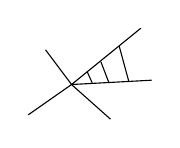
\begin{tikzpicture}[scale=.55]
\draw (-1,-.7)--(0,0)--(.9,-.8) (0,0)--(-.6,.8) (0,0)--(1.6,1.3) (0,0)--(1.85,.1);
\draw (.48,.03)--(.36,.3) (.86,.05)--(.68,.52) (1.32,.08)--(1.1,.89);
\end{tikzpicture}}

\diagram{\begin{tikzcd}[ampersand replacement=\&,row sep=tiny,column sep=tiny]
\&\&\bullet\arrow[dl]\&\bullet\arrow[l]\arrow[d]\\
\&\bullet\&\&\bullet\arrow[ll]\\
\bullet\arrow[ur]\&\&\bullet\arrow[ul]\&\\
\&\bullet\arrow[ul]\arrow[ur]\&\&
\end{tikzcd}}

a) $\forall f\in F$, les $s\in S$ et $a\in A$ incidents \unsure{à|:} $f$ forment un polygône, donc

a) Si $a<f$ ($a\in A$) $a$ a \unsure{exact\textsuperscript{t}} 2 sommets

\figure{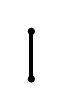
\begin{tikzpicture}[scale=.55]\draw[line width=1.4pt](0,0)--(0,1.1);\fill (0,0) circle (.085) (0,1.1) circle (.085);\end{tikzpicture}}

b) Si $s<f$ ($s\in S$) il y a \unsure{exact\textsuperscript{t}} 2 arêtes entre $s$ et $f$)

c) Condition de connexité

\figure{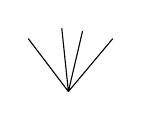
\begin{tikzpicture}[scale=.6]\draw (0,0)--(-.85,1.12) (0,0)--(-.14,1.34) (0,0)--(.3,1.28) (0,0)--(.94,1.12);\end{tikzpicture}}

\diagram{\begin{tikzcd}[ampersand replacement=\&,row sep=tiny,column sep=tiny]
\&\unsure{\omega|s}\&\&\unsure{\bar s|s'|\bar 3}\arrow[ll]\\
\&\bullet\&\unsure{s}\arrow[l]\&\bullet\arrow[l]\\
\unsure{\bar s|s|-a}\arrow[ur]\&\deleted{\unsure{s}}\arrow[u]\&\unsure{\bar s|s'|\bar 3}\arrow[u]\&s\arrow[u]\arrow[uu]\\
\&\underset{\unsure{a|x|\bullet}}{\bullet}\arrow[ul]\arrow[u]\arrow[ur]\arrow[urr]\&\&
\end{tikzcd}}

On trouve aussi que \unsure{tte|les} arête est incidente à une face (\unsure{sinon} on aurait ds $|\mathcal X|$ des pts au voisinage desquels $|\mathcal X|$ est de dim $1$ !) et \deleted{\unsure{on trouve que}}\inserted{on en conclut} que \uline{tte} \uline{arête} a \unsure{exact\textsuperscript{t}} 2 sommets\ldots

\figure{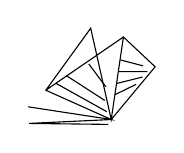
\begin{tikzpicture}[scale=.62]
\draw (0,0)--(-1.34,.6)--(-.42,1.87)--(0,0)--(.25,1.69)--(.9,1.08)--(0,0)
(-1.34,.6)--(.25,1.69) (-1.34,.6)--(0,0)--(-1.7,.26) (0,0)--(-1.68,-.08)--(-.06,-.1);
\draw (-1.13,.74)--(-.09,.16) (-.92,.9)--(-.13,.39) (-.46,1.14)--(-.11,.67)
(.08,.51)--(.51,.72) (.12,.74)--(.64,.87) (.16,.98)--(.74,.98) (.19,1.22)--(.65,1.1);
\end{tikzpicture}}
}

en faisant opérer $\sigma_{n-1},\ldots,\sigma_{p+1}$ trivialement sur $R_p$ \quad ($n\unsure{>|{\ge}}p\ge0$)

\figure{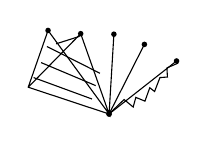
\begin{tikzpicture}[scale=.68]
\draw (0,0)--(-1.51,.5)--(-1.14,1.56)--(0,0)--(-.53,1.5)--(-1.51,.5)
(0,0)--(.09,1.49) (0,0)--(.66,1.3) (0,0)--(1.26,.99);
\draw (-1.41,.68)--(-.32,.28) (-1.27,.96)--(-.25,.53) (-1.16,1.26)--(-.17,.76) (-.99,1.31)--(-.55,1.45);
\draw (0,0)--(.28,.27)--(.45,.13)--(.5,.31)--(.67,.24)--(.76,.49)--(.85,.42)--(.95,.68)--(1.09,.69)--(1.08,.86)--(1.29,.95);
\fill (0,0) circle (.055) (-1.14,1.56) circle (.052) (-.53,1.5) circle (.052) (.09,1.49) circle (.052) (.66,1.3) circle (.052) (1.26,.99) circle (.052);
\end{tikzpicture}}

% archive sheet number: 40
